\documentclass{standalone}
\usepackage{tikz}

\begin{document}

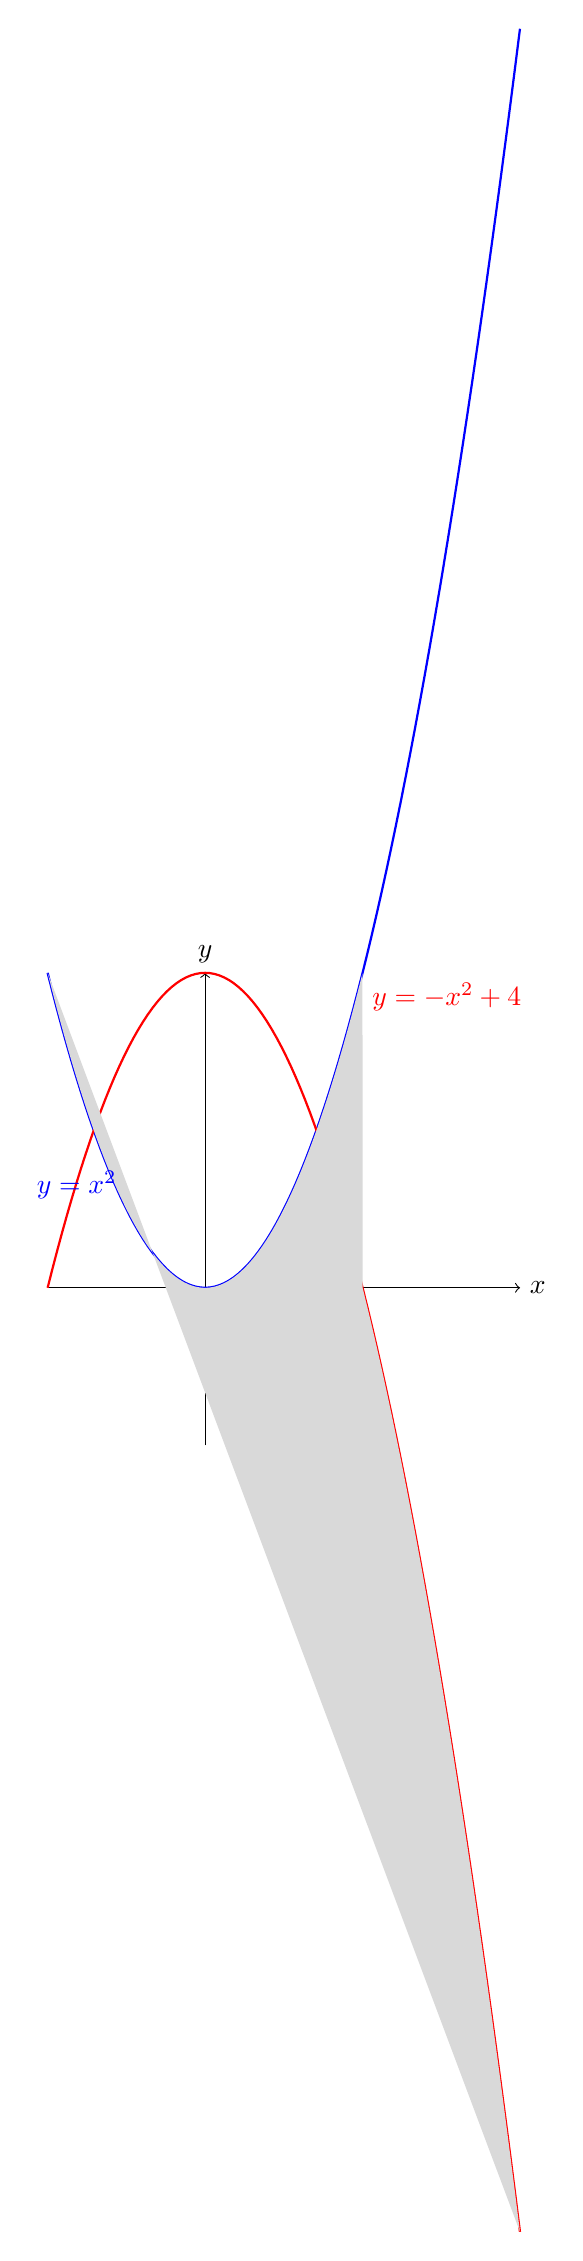
\begin{tikzpicture}[scale=1]
    % Define the domain and step size for the plots
    \def\xmin{-2}
    \def\xmax{4}
    \def\step{0.1}

    % Draw the axes
    \draw[->] (\xmin,0) -- (\xmax,0) node[right] {$x$};
    \draw[->] (0,-2) -- (0,\xmax) node[above] {$y$};

    % Draw the blue curve (e.g., y = x^2)
    \draw[blue, thick] plot[domain=\xmin:\xmax, samples=100] (\x, {pow(\x, 2)});

    % Draw the red curve (e.g., y = -x^2 + 4)
    \draw[red, thick] plot[domain=\xmin:\xmax, samples=100] (\x, {-pow(\x, 2) + 4});

    % Fill the area between the two curves
    \fill[gray!30] plot[domain=\xmin:2, samples=100] (\x, {pow(\x, 2)}) -- plot[domain=2:\xmax, samples=100] (\x, {-pow(\x, 2) + 4}) -- cycle;

    % Label the curves
    \node at (2, 4) [below right] {\color{red} $y = -x^2 + 4$};
    \node at (-1, 1) [above left] {\color{blue} $y = x^2$};
\end{tikzpicture}

\end{document}